%%%%%%%%%%%%%%%%%%%%%%%%%%%%%%%%%%%%%%%%%%%%%%%%%%%%%%%%%%%%%%%%%%
%%%%%%%% ICML 2013 EXAMPLE LATEX SUBMISSION FILE %%%%%%%%%%%%%%%%%
%%%%%%%%%%%%%%%%%%%%%%%%%%%%%%%%%%%%%%%%%%%%%%%%%%%%%%%%%%%%%%%%%%

% Use the following line _only_ if you're still using LaTeX 2.09.
%\documentstyle[icml2013,epsf,natbib]{article}
% If you rely on Latex2e packages, like most moden people use this:
\documentclass{article}

% For figures
\usepackage{graphicx} % more modern
%\usepackage{epsfig} % less modern
\usepackage{subfigure} 

% For citations
\usepackage{natbib}

% For algorithms
\usepackage{algorithm}
\usepackage{algorithmic}

% As of 2011, we use the hyperref package to produce hyperlinks in the
% resulting PDF.  If this breaks your system, please commend out the
% following usepackage line and replace \usepackage{icml2013} with
% \usepackage[nohyperref]{icml2013} above.
\usepackage{hyperref}

% Packages hyperref and algorithmic misbehave sometimes.  We can fix
% this with the following command.
\newcommand{\theHalgorithm}{\arabic{algorithm}}

% Employ the following version of the ``usepackage'' statement for
% submitting the draft version of the paper for review.  This will set
% the note in the first column to ``Under review.  Do not distribute.''
\usepackage{icml2013} 
% Employ this version of the ``usepackage'' statement after the paper has
% been accepted, when creating the final version.  This will set the
% note in the first column to ``Proceedings of the...''
%\usepackage[accepted]{icml2013}


% The \icmltitle you define below is probably too long as a header.
% Therefore, a short form for the running title is supplied here:
\icmltitlerunning{Submission and Formatting Instructions for ICML 2013}

\begin{document} 

\twocolumn[
\icmltitle{Twitter Trend Detection and Classification}

% It is OKAY to include author information, even for blind
% submissions: the style file will automatically remove it for you
% unless you've provided the [accepted] option to the icml2013
% package.
\icmlauthor{Your Name}{email@yourdomain.edu}
\icmladdress{Your Fantastic Institute,
            314159 Pi St., Palo Alto, CA 94306 USA}
\icmlauthor{Your CoAuthor's Name}{email@coauthordomain.edu}
\icmladdress{Their Fantastic Institute,
            27182 Exp St., Toronto, ON M6H 2T1 CANADA}

% You may provide any keywords that you 
% find helpful for describing your paper; these are used to populate 
% the "keywords" metadata in the PDF but will not be shown in the document
\icmlkeywords{boring formatting information, machine learning, ICML}

\vskip 0.3in
]

\begin{abstract} 
There are three review cycles for ICML 2013, with full paper submissions 
due on October 1, 2012; December 15, 2012; and February 15, 2013. Reviewing 
will be blind to the identities of the authors, and therefore identifying
information must not appear in any way in papers submitted for review. 
Submissions must be in PDF, with an 8 page length limit (upto 9 pages 
including references).
\end{abstract} 

\section{Introduction}
\label{submission}



\section{Related Work} 
The paper \cite{nikolov2012trend} introduced a new approach to detecting Twitter trends in a nonparametric method. It presented a general time series analysis method that can be used to detect the future trend on twitter. This paper used both positive trending examples and negative, or non-trending example to vote for the current observation sequence. Then based on the voting result to find out whether it's a trend or not. The result of this paper is fairly good. In 79\% percent of cases, this paper detected trending topics earlier than Twitter (1.43 hours earlier), and it managed to keep an error rate of around 95\% (4\% false positive rate, 95\% true positive rate). As this paper's experiment result shows that it is fairly good to use time series data to predict trends in twitter, we believe the time series prior of the peak would be a good indictor of the trend pattern.
 
The paper \cite{journals/corr/abs-1102-1402} made a detail analysis on different kinds of factors that may affect the persistence and decay of twitter trend based on history data and experiments. It showed that the resonance of the content with the users of the social network plays a major role in causing trends.It also demonstrate empirically how factors such
as user activity and number of followers do not contribute strongly to trend creation and its propagation. Based on the conclusion of this paper, we believe that content of twitter activity has a major influence to the type of twitter trends.
\section{Dataset} 


\section{Method}

Twitter trends are measured by the activity of Twitter hashtags or topics. In our work, we use the activity of hashtag to measure Twitter trend. We want to predict the future trend of an emerging hashtag/topic based on either content or some previous temporal information from tweets containing that hashtag. For example, we want to predict future trend of hashtag "\#protest" based on some previous tweets containing that hashtag, like \texttt{"RT Iranian women must liberate themselves http://rurl.org/1rlv \#protest \#nytimes"}.

The problem can be approached as a supervised learning problem. We first assign each hashtag a trending pattern based on its time series. Although this problem is a supervised learning problem, we label the instances through clustering. From then on, we can train a classifier based on either text content or time series from hashtag histogram. And we could then classify the hashtag to different patterns using our classifier. 

The content and temporal information maybe beneficial in predicting the trend pattern of a hashtag. We use content information because some words or phrases reveal their trend to some extent. For example, the trend pattern of "\#olympics" is different from "\#apple" that "\#olympics" is reoccurring every four years and it will only be a trend when it is going on, while "\#apple" is a daily trend and can trigger a trend very often like it has new product to release or new dispute with competitors. The context words associate with "\#olympics", like athlete names "Michael Phelps" and medals "Gold Medal", and "\#apple", like product name "iPhone" and competitor name "Samsung", are quite informative when training and testing using classifiers. We also use temporal information like the time series (histogram volume) as an another way to predict trend. The ups and downs in different time series can also indicate different patterns.      

In our paper, we have used K-SC algorithm to do Trend Clustering of time series \cite{Yang11}. We have tried four different approaches to do Trend Prediction.  

\subsection{Trend Clustering}

We do Trend Clustering mainly to label the data, which assign a label to a time series according to which cluster it belongs. We use these labeled data to do training and testing on our classifiers. 

We use the K-SC algorithm \cite{Yang11} to do clustering of the 128 hours time series with peak located at 1/3 of the 128 hours. This algorithm is very similar to K-means algorithm. It has for each data points calculate which nearest cluster centroid it belongs and then compute the new cluster centroid again. The only two differences with K-means are K-SC uses the special designed similarity metric, which is similar to Time Wrapping Distance (compute distance after shifting and scaling). Another difference is K-SC uses a new method to compute cluster centroid, which is essentially select the centroid that minimize the squared distance over all data points to their closest centroid using the new similarity metric.     

We choose to K=6 and the clustering result in Figure~\ref{six-cluster}

\begin{figure}[ht]
\vskip 0.2in
\begin{center}
\centerline{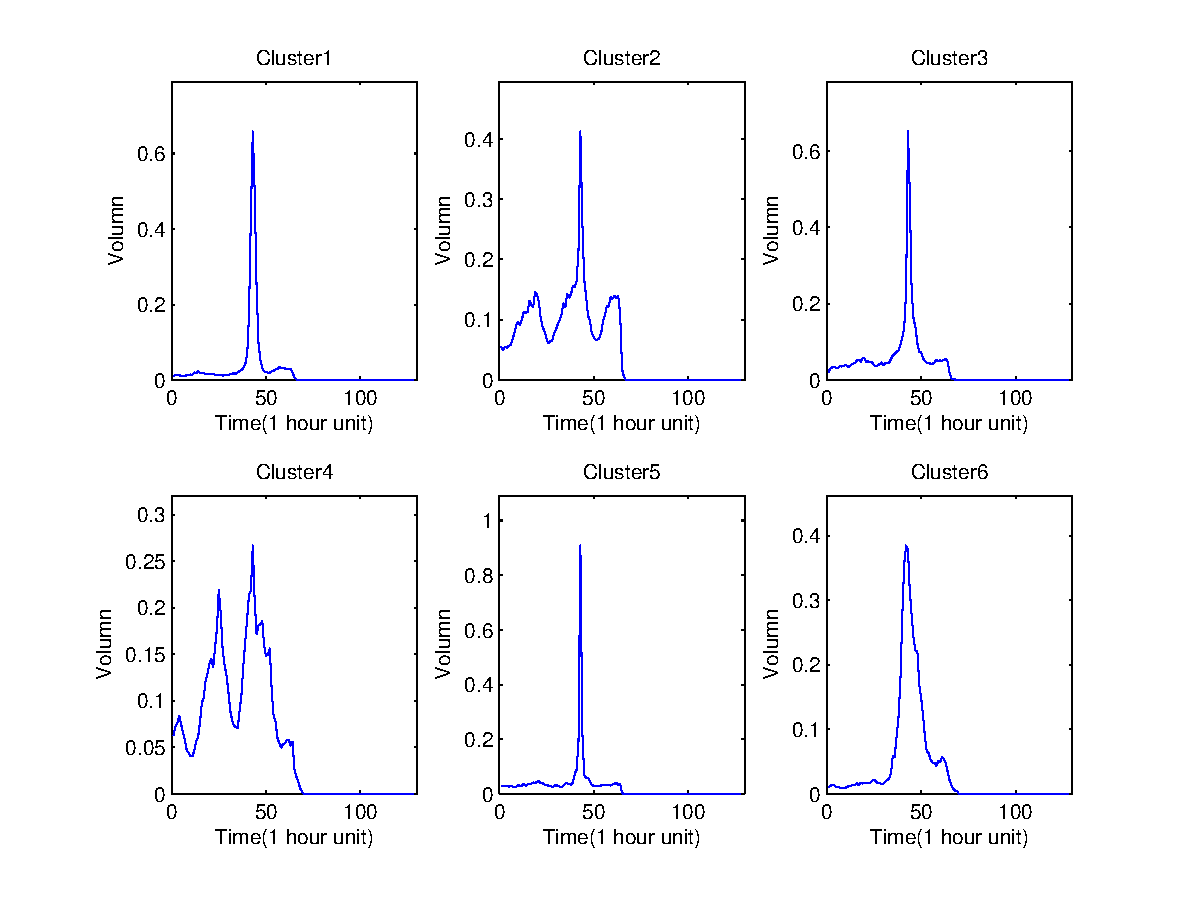
\includegraphics[width=\columnwidth]{sixClusters}}
\caption{All model performance using different metrics.}
\label{six-cluster}
\end{center}
\vskip -0.2in
\end{figure} 

\subsection{Trend Prediction}

For predicting Twitter trend, we can consider using both content information and temporal information as the clue for the trending activity.   

\subsubsection{Bag-of-Word Naive Bayes Trend Prediction}
The Naive Bayes Method is the first one we come up with in this project. Since this is a classification problem and tweets are composed of words and tokens, the use of bag of word model is very intuitive. The Naive Bayes algorithm we implemented is similar to the one we did in homework. For the training set, each tweet has a label (1 to 6), so each of them can be treated as a training sample. We first utilize LingPipe to tokenize the tweets by considering lowercase, stemming, etc. Then with these separate tokens, we count the number of co-occurrence and other metrics needed to build the Naive Bayes model. The whole process was done very quickly and efficiently using Hadoop.
After getting all the model parameters we need, we start working on the test data. The log likelihood of each test sample can be written as:
\begin{equation} 
(\prod_{j=1}^d  \frac{C(X_j=x_j \wedge Y=y')+mq_j}{C(Y=y')+m})\frac{C(Y=y')+mq_j}{C(Y=ANY)+m}
\end{equation}
Using this equation, we can easily classify our test tweets data into one of the six categories. But here we made some changes on the test process. We first combine several tweets of the same hashtag into one document, then apply the NB classifiers. The reason we did so is because the tweets are often very short, thus making the token distribution very sparse which may lead to bad result. 

In addition to this traditional Naive Bayes method, we also take the weight of token into account. We believe that some of the words must be more important than others when apply to certain situations or categories. For example, people won't talk about Hurricane too often usually, but when we have a real Hurricane in the world, the world Hurricane becomes important. To discover such important tokens and give different weight on them, we first calculate both background and foreground token distributions, and use Chi-square method to find those important words. The Chi-Square method can be written as

\begin{equation} 
\frac{(fg-bg)^2}{bg}
\end{equation}

By using this model, we successfully find out those important words give certain cluster. For example, in cluster 3, the top 10 words include mac, apple, ipad, ipod, chrome, android, etc., which are all relevant to IT fields. Though this token weight makes sense, when apply to Naive Bayes Model, we didn't find good improvement on the final results. Maybe our combine method is not good enough, which we may dig deeper later.

\subsubsection{Bag-of-Word Logistic Regression Trend Prediction}

In trend prediction using bag-of-word Logistic Regression, we treat all words in the tweets containing the hashtag as a document (bag-of-word). The document's label is the hashtag's label assigned in Trend Clustering part based on the clustering result from hashtag's time series. For this specific Logistic Regression problem, we want to maximize log likelihood $L(w)=\Pi_lP(y^l|x^l,w)$, where $x^l$ represents the $l$th training document (BOW of all words in tweets containing the same hashtag), $y^l$ represents the class label of $l$th training document and $w$ is the model weight. Using stochastic gradient descent, we can derive the training rules as 

\begin{equation} 
w_{ij}=w_{ij} + \lambda(y^l - \hat{y}^l) x^l - 2\lambda \mu w_{ij} \label{eq:lrtrain}
\end{equation}

where $w_{ij}$ is the $i$th classifier's $j$th element in weight vector, $y^l$ is the true class label of $l$th training document, $\hat{y}^l$ is the predicted probability of chewing this label as the class label of $l$th training document, $x^l$ is the bag-of-words in $l$th training document,  $\lambda$ is the gradient step size, $\mu$ is the regularization constant. To make our algorithm more fast and space efficient for processing large data, we use the delayed update stochastic gradient descend with hash trick that introduced in class. 

Since this specific Logistic Regression classifier is a multi class classifier, we train multiple binary classifier and choose the label with the largest weight in the test phase. The testing document consists of bag-of-words all words in tweets containing the same hashtag. The test rules is    

\begin{equation} 
y^l =\arg\max_i  \sum_j w_{ij} x_j^l\label{eq:lrtest}
\end{equation}

where $w_{ij}$ is the $i$th classifier's $j$th element in weight vector, $y^l$ is the predicted class label for $l$th testing instance, $x_j^l$ is the $j$th word (feature after hash trick) in $l$th testing document. 

\subsubsection{Time Series Similarity Measurement}
After working on content based measurement of  Twitter trend, we turn to use temporal information with hashtag to classify and predict the type of Twitter trend. Based on the former research\cite{nikolov2012trend} about the twitter trend,
we believe time series prior of the peak would be a good indictor of the trend pattern. So we add this part time series information to do classification and prediction.
Different from \cite{nikolov2012trend}, we not only need to predict if the sequence of tweets will be a trend, but also decide which trend pattern it would be. The meaning of doing this is find the spread pattern of twitter trend before the trend reaches its peak.  Because of time limitation, we applied a parametric model to predict and classify the trend pattern instead of using a nonparametric prediction. The whole process could be divided into two steps. Trend prediction and Trend classification.

The trend prediction is find the twitter activity that could become a trend. We can assume that a normal trend model of tweet activity is roughly constant with occasional jumps. So the detection process is similar with a filter, which is used to filter the occasional jump and find the true jump that become a twitter trend.

Here we define a trend by two variables, jump rate and popularity duration. Jump rate is 
\begin{equation} 
\frac{\alpha * standard variance}{mean}
\end{equation}
The standard variance and mean refer to the twitter activity of the according time interval.
Popularity duration is the total volume in a time interval. If the popularity duration is beta times higher than the mean popularity duration value. We will consider this is a trend. As this is a parametric model, alpha and beta needs to be estimated by experiment. When monitoring the twitter activity, we use a sliding window to check if current trend would become a twitter trend. A acceleration step applied here that we don't need to compute the parametric model every hour but only when the twitter activity has a large increase. 
The above detection process is illustrated in Figure~\ref{imgjump}.
\begin{figure}[ht]
\vskip 0.2in
\begin{center}
\centerline{\includegraphics[width=\columnwidth]{jump}}
\caption{The detection of a big jump}
\label{imgjump}
\end{center}
\vskip -0.2in
\end{figure} 
When the sliding window comes  to a beginning of trend, we can see in the red box, the jump rate and popularity duration is satisfied by the parametric model. We will consider this is a big jump, which imply the follow twitter activity will become a trend. Then we will come to the classification step to decide the type of the possible trend.

In the above step, we already get the trend patterns. So we apply a similarity measurement to classify the pattern of possible trend. As this twitter time series activity is discrete data, we compute the similarity of current twitter activity to each patterns for each hour. In another words, each hour in the time interval will vote for each trend pattern based on similarity between the instance in detected time interval and trend patterns.
The similarity is defined by a decaying exponential, in this form, the nearest time series data has more weights while the non-similar data has less weight. Similarity defined as follows:
\begin{equation} 
Similarity(instance, pattern) = e^{-d(i, p)}
\end{equation}
In the above equation, i means the time series data at time i. p means the detected pattern time series data in the according time i. d(i, p) is the euclidean distance between i and p. The similarity measurement process is illustrated in figure ~\ref{imgcmp}
\begin{figure}[ht]
\vskip 0.2in
\begin{center}
\centerline{\includegraphics[width=\columnwidth]{compare}}
\caption{Illustration of similarity measurement process}
\label{imgcmp}
\end{center}
\vskip -0.2in
\end{figure} 
The left subfigure in figure~\ref{imgcmp} is a section of twitter activity of certain hashtag, which is the time series data of 8 month. We can see that there could be several small jumps leading up to a big jump. The right subfigure in figure~\ref{imgcmp} is a detected pattern of twitter trend, which is the time series data of 128 hours of all twitter activity in this pattern.  


\subsubsection{Time Series Logistic Regression Trend Prediction}

Although bag-of-words model can give us some hints about future trend, using content information to predict temporal pattern is somewhat limited. Because words alone are not always correlated with trend. Therefore, we use directly a time interval in time series (hashtag histogram) to predict the future trend pattern. 

Since we have clustered the time series using the 128 hours time series, placing the peak at one third in the whole 128 hours time series, we assume that the time interval prior to a trend (0-43 hour) is a good indicator of future pattern of trend. We define trend as a sudden jump in the time series here. Therefore, we still model the problem as a classification problem that we can train and test using Logistic Regression based on the data points in a short interval that in the very beginning of time series. 

We always choose the interval prior to a trend (sudden jump in time series) to train and test, since we want to predict the future pattern of trend as quickly as possible with least amount of previous known data. Therefore, the problem becomes to detect trend and use the interval of time series when the trend just begin gaining popularity to train and test our classifier. We can then try to solve the transformed problems with two assumptions here: predict trend patterns with known trend and predict trend patterns with unknown trend. 

{\bf Predict Trend Patterns with Known Trend:} We use the only trend that leads to peak (sudden jump in highest time series globally) in time series as the best trend as the interval for training and testing. With known most salient trend, we could get more good training instances and thus good classifier which leads to better testing results.

{\bf Predict Trend Patterns with Unknown Trend:} We now need to detect a relative good trend (sudden jump in highest time series locally) by our trend detection algorithm. The detection algorithm needs to find real potential trend instead of small fluctuations. The algorithm is parametric that it needs parameter tuning to avoid this. 






\section{Experiment} 

\subsection{Data Preparation}

We extract nearly 200 million tweets from Brendan's "Gardenhose" archive from June 2009 to February 2010 as same time period as described in the paper \cite{Yang11}. And we further extract 2.5 million all the tweets containing the top 998 most frequently appeared hashtags. This data size is ~600MB compressed and >3GB uncompressed.  

Besides that, we also build our time series based on the number of tweets in each one hour unit. For the known peak time series, we build time series using the truncated time series of 128 hours with peak located at the 1/3 of the 128 hours. For the unknown peak time series, we build time series throughout the whole eight months. 

\subsection{Content (BOW) vs Temporal (Time Series)}

We can see from Table~\ref{tab-result} the final evaluation result from the table below. Note that ``BOW\_NB" and ``BOW\_LR" represents Naive Bayes and Logistic Regression using Bag-of-Word model respectively. ``TS\_LR\_KT" and ``TS\_LR\_UNKT" represents Logistic Regression with known trend and unknown trend using time series model respectively. The time series model only have trained and tested using only a interval of nine data points (first nine hours of a trend which the popularity is about to go up).  

\begin{table}[t]
\caption{Model performance using different metrics}
\label{tab-result}
\vskip 0.15in
\begin{center}
\begin{small}
\begin{sc}
\begin{tabular}{lcccr}
\hline
\abovespace\belowspace
Model Name & Precision & Recall & F-measure \\
\hline
\abovespace
BOW\_NB   & 0.22 & 0.22 & 0.22 \\		
BOW\_LR & 0.34 & 0.13 & 0.19 \\		
TS\_LR\_KT    & \textbf{0.57} & \textbf{0.57} & \textbf{0.57} \\	
TS\_LR\_UNKT   & 0.31 & 0.34 & 0.33     \\
TS\_SM\_UNKT	& 0.19	& 0.19	& 0.19	\\
\belowspace
TS\_LR\_UNKT	& 0.31	& 0.34	& 0.33	\\
\hline
\end{tabular}
\end{sc}
\end{small}
\end{center}
\vskip -0.1in
\end{table}

\begin{figure}[ht]
\vskip 0.2in
\begin{center}
\centerline{\includegraphics[width=\columnwidth]{allPerformance}}
\caption{All model performance using different metrics.}
\label{all-performance}
\end{center}
\vskip -0.2in
\end{figure} 


As we can see from Figure~\ref{all-performance}, we can see that the time series based model gives us way more better performance than content based model (TS is much better than BOW). The reason might be tweets content can only provide little information about the trend of the underlying topic they talk about. Or we haven't found a better way to use the content data.

Besides, Logistic Regression (LR) classifier works better than Naive Bayes (NB) classifier in content based Bag-of-Word model. This is not surprising that LR works better than NB, since NB assume the oder of words does't not matter, namely independence among a sequence of words. 


\subsection{Known vs Unknown Trend}

As shown in Figure~\ref{all-performance}, we can run our classification algorithm on both previous known trend (tested on 128 hours time series and regard the interval around peak as most salient trend) and unknown trend (tested on 8 months time series and detected most salient trend by our detection algorithm). We can see from the figure below that the Precision, Recall and F-measure became worse when we switch to use our own trend detection algorithm. 

This indicates that with a better trend detection algorithm, we can use the real time streaming data to predict a trend and a future hottest emerging trending pattern to a specific hashtag/topic. 


\section{Conclusion} 
Tweet content has a big connection with tweet trend patterns. But the key information for this is difficult to extract.  
Temporal information is the direct representation of tweet trend and the time interval prior to a trend is a good indicator of future pattern of trend. 



\subsection{Templates for Papers}

Electronic templates for producing papers for submission are available
for \LaTeX\/ and Microsoft Word. Templates are accessible on the World
Wide Web at:\\
\textbf{\texttt{http://icml.cc/2013/}}

\noindent
Send questions about these electronic templates to
\texttt{program@icml.cc}.

The formatting instructions below will be enforced for initial submissions and camera-ready copies. 
\begin{itemize}
\item The maximum paper length is 8 pages excluding references, and 
9 pages including references.
\item Do not alter the style template; in particular, do not compress the paper format 
by reducing the vertical spaces.
\item Do not include author information or acknowledgments in your
  initial submission. 
\item Place figure captions {\em under} the figure (and omit titles from
  inside the graphic file itself).  Place table captions {\em over}
  the table.
\item References must include page numbers whenever possible and be as
  complete as possible.  Place multiple citations in chronological order.  
\end{itemize}
Please see below for details on each of these items.

\subsection{Submitting Papers}

Submission to ICML 2013 will be entirely electronic, via a web site
(not email).  The URL and information about the submission process
are available on the conference web site at

\textbf{\texttt{http://icml.cc/2013/}}

{\bf Paper Deadline:} The deadline for paper submission to ICML 2013
is at 23:59 Universal Time (3:59 Pacific Daylight Time) on the due date
(October 1, December 15, or February 15, depending on the review cycle).  
If your full submission does not reach us by this time, it will 
not be considered for publication. There is no separate abstract submission.

{\bf Anonymous Submission:} To facilitate blind review, no identifying
author information should appear on the title page or in the paper
itself.  Section~\ref{author info} will explain the details of how to
format this.

{\bf Simultaneous Submission:} ICML will not accept any paper which,
at the time of submission, is under review for another conference or
has already been published. This policy also applies to papers that
overlap substantially in technical content with conference papers
under review or previously published. ICML submissions must not be
submitted to other conferences during ICML's review period. Authors
may submit to ICML substantially different versions of journal papers
that are currently under review by the journal, but not yet accepted
at the time of submission. Informal publications, such as technical
reports or papers in workshop proceedings which do not appear in
print, do not fall under these restrictions.

\medskip

To ensure our ability to print submissions, authors must provide their
manuscripts in \textbf{PDF} format.  Furthermore, please make sure
that files contain only Type-1 fonts (e.g.,~using the program {\tt
  pdffonts} in linux or using File/DocumentProperties/Fonts in
Acrobat).  Other fonts (like Type-3) might come from graphics files
imported into the document.

Authors using \textbf{Word} must convert their document to PDF.  Most
of the latest versions of Word have the facility to do this
automatically.  Submissions will not be accepted in Word format or any
format other than PDF. Really. We're not joking. Don't send Word.

Those who use \textbf{\LaTeX} to format their accepted papers need to
pay close attention to the typefaces used.  Specifically, when
producing the PDF by first converting the dvi output of \LaTeX\ to Postscript
the default behavior is to use non-scalable Type-3 PostScript bitmap
fonts to represent the standard \LaTeX\ fonts. The resulting document
is difficult to read in electronic form; the type appears fuzzy. To
avoid this problem, dvips must be instructed to use an alternative
font map.  This can be achieved with
something like the following commands:\\[0.5em]
{\bf dvips -Ppdf -tletter -G0 -o paper.ps paper.dvi}\\
{\bf ps2pdf paper.ps}\\[0.5em]
Note that it is a zero following the ``-G''.  This tells dvips to use
the config.pdf file (and this file refers to a better font mapping).

Another alternative is to use the \textbf{pdflatex} program instead of
straight \LaTeX. This program avoids the Type-3 font problem, however
you must ensure that all of the fonts are embedded (use {\tt
pdffonts}). If they are not, you need to configure pdflatex to use a
font map file that specifies that the fonts be embedded. Also you
should ensure that images are not downsampled or otherwise compressed
in a lossy way.

Note that the 2013 style files use the {\tt hyperref} package to
make clickable links in documents.  If this causes problems for you,
add {\tt nohyperref} as one of the options to the {\tt icml2013}
usepackage statement.

\subsection{Reacting to Reviews}
We will continue the ICML tradition in which the authors are given the
option of providing a short reaction to the initial reviews. These
reactions will be taken into account in the discussion among the
reviewers and area chairs.

\subsection{Submitting Final Camera-Ready Copy}

The final versions of papers accepted for publication should follow the
same format and naming convention as initial submissions, except of
course that the normal author information (names and affiliations)
should be given.  See Section~\ref{final author} for details of how to
format this.

The footnote, ``Preliminary work.  Under review by the International
Conference on Machine Learning (ICML).  Do not distribute.'' must be
modified to ``\textit{Proceedings of the
$\mathit{30}^{th}$ International Conference on Machine Learning},
Atlanta, Georgia, USA, 2013.  JMLR: W\&CP volume 28. 
Copyright 2013 by the author(s).''

For those using the \textbf{\LaTeX} style file, simply change
$\mathtt{\backslash usepackage\{icml2013\}}$ to 

\verb|\usepackage[accepted]{icml2013}|

\noindent
Authors using \textbf{Word} must edit the
footnote on the first page of the document themselves.

Camera-ready copies should have the title of the paper as running head
on each page except the first one.  The running title consists of a
single line centered above a horizontal rule which is $1$ point thick.
The running head should be centered, bold and in $9$ point type.  The
rule should be $10$ points above the main text.  For those using the
\textbf{\LaTeX} style file, the original title is automatically set as running
head using the {\tt fancyhdr} package which is included in the ICML
2013 style file package.  In case that the original title exceeds the
size restrictions, a shorter form can be supplied by using

\verb|\icmltitlerunning{...}|

just before $\mathtt{\backslash begin\{document\}}$.
Authors using \textbf{Word} must edit the header of the document themselves.
 
All submissions must follow the same format to ensure the printer can
reproduce them without problems and to let readers more easily find
the information that they desire.

\subsection{Length and Dimensions}

Papers must not exceed eight (8) pages, including all figures, tables,
and appendices, but excluding references. When references are included,
the paper must not exceed nine (9) pages. Any submission that exceeds 
this page limit or that diverges significantly from the format specified 
herein will be rejected without review.

The text of the paper should be formatted in two columns, with an
overall width of 6.75 inches, height of 9.0 inches, and 0.25 inches
between the columns. The left margin should be 0.75 inches and the top
margin 1.0 inch (2.54~cm). The right and bottom margins will depend on
whether you print on US letter or A4 paper, but all final versions
must be produced for US letter size.

The paper body should be set in 10~point type with a vertical spacing
of 11~points. Please use Times Roman typeface throughout the text.

\subsection{Title}

The paper title should be set in 14~point bold type and centered
between two horizontal rules that are 1~point thick, with 1.0~inch
between the top rule and the top edge of the page. Capitalize the
first letter of content words and put the rest of the title in lower
case.

\subsection{Author Information for Submission}
\label{author info}

To facilitate blind review, author information must not appear.  If
you are using \LaTeX\/ and the \texttt{icml2013.sty} file, you may use
\verb+\icmlauthor{...}+ to specify authors.  The author information
will simply not be printed until {\tt accepted} is an argument to the
style file. Submissions that include the author information will not
be reviewed.

\subsubsection{Self-Citations}

If your are citing published papers for which you are an author, refer
to yourself in the third person. In particular, do not use phrases
that reveal your identity (e.g., ``in previous work \cite{langley00}, we 
have shown \ldots'').

Do not anonymize citations in the reference section by removing or
blacking out author names. The only exception are manuscripts that are
not yet published (e.g. under submission). If you choose to refer to
such unpublished manuscripts \cite{anonymous}, anonymized copies have 
to be submitted
as Supplementary Material via CMT. However, keep in mind that an ICML
paper should be self contained and should contain sufficient detail
for the reviewers to evaluate the work. In particular, reviewers are
not required to look a the Supplementary Material when writing their
review.

\subsubsection{Camera-Ready Author Information}
\label{final author}

If a paper is accepted, a final camera-ready copy must be prepared.
%
For camera-ready papers, author information should start 0.3~inches
below the bottom rule surrounding the title. The authors' names should
appear in 10~point bold type, electronic mail addresses in 10~point
small capitals, and physical addresses in ordinary 10~point type.
Each author's name should be flush left, whereas the email address
should be flush right on the same line. The author's physical address
should appear flush left on the ensuing line, on a single line if
possible. If successive authors have the same affiliation, then give
their physical address only once.

A sample file (in PDF) with author names is included in the ICML2013 
style file package.

\subsection{Abstract}

The paper abstract should begin in the left column, 0.4~inches below
the final address. The heading `Abstract' should be centered, bold,
and in 11~point type. The abstract body should use 10~point type, with
a vertical spacing of 11~points, and should be indented 0.25~inches
more than normal on left-hand and right-hand margins. Insert
0.4~inches of blank space after the body. Keep your abstract brief and 
self-contained,
limiting it to one paragraph and no more than six or seven sentences.

\subsection{Partitioning the Text} 

You should organize your paper into sections and paragraphs to help
readers place a structure on the material and understand its
contributions.

\subsubsection{Sections and Subsections}

Section headings should be numbered, flush left, and set in 11~pt bold
type with the content words capitalized. Leave 0.25~inches of space
before the heading and 0.15~inches after the heading.

Similarly, subsection headings should be numbered, flush left, and set
in 10~pt bold type with the content words capitalized. Leave
0.2~inches of space before the heading and 0.13~inches afterward.

Finally, subsubsection headings should be numbered, flush left, and
set in 10~pt small caps with the content words capitalized. Leave
0.18~inches of space before the heading and 0.1~inches after the
heading. 

Please use no more than three levels of headings.

\subsubsection{Paragraphs and Footnotes}

Within each section or subsection, you should further partition the
paper into paragraphs. Do not indent the first line of a given
paragraph, but insert a blank line between succeeding ones.
 
You can use footnotes\footnote{For the sake of readability, footnotes
should be complete sentences.} to provide readers with additional
information about a topic without interrupting the flow of the paper. 
Indicate footnotes with a number in the text where the point is most
relevant. Place the footnote in 9~point type at the bottom of the
column in which it appears. Precede the first footnote in a column
with a horizontal rule of 0.8~inches.\footnote{Multiple footnotes can
appear in each column, in the same order as they appear in the text,
but spread them across columns and pages if possible.}

\begin{figure}[ht]
\vskip 0.2in
\begin{center}
\centerline{\includegraphics[width=\columnwidth]{icml_numpapers}}
\caption{Historical locations and number of accepted papers for International
  Machine Learning Conferences (ICML 1993 -- ICML 2008) and
  International Workshops on Machine Learning (ML 1988 -- ML
  1992). At the time this figure was produced, the number of
  accepted papers for ICML 2008 was unknown and instead estimated.}
\label{icml-historical}
\end{center}
\vskip -0.2in
\end{figure} 

\subsection{Figures}
 
You may want to include figures in the paper to help readers visualize
your approach and your results. Such artwork should be centered,
legible, and separated from the text. Lines should be dark and at
least 0.5~points thick for purposes of reproduction, and text should
not appear on a gray background.

Label all distinct components of each figure. If the figure takes the
form of a graph, then give a name for each axis and include a legend
that briefly describes each curve. Do not include a title inside the
figure; instead, the caption should serve this function.

Number figures sequentially, placing the figure number and caption
{\it after\/} the graphics, with at least 0.1~inches of space before
the caption and 0.1~inches after it, as in
Figure~\ref{icml-historical}.  The figure caption should be set in
9~point type and centered unless it runs two or more lines, in which
case it should be flush left.  You may float figures to the top or
bottom of a column, and you may set wide figures across both columns
(use the environment {\tt figure*} in \LaTeX), but always place
two-column figures at the top or bottom of the page.

\subsection{Algorithms}

If you are using \LaTeX, please use the ``algorithm'' and ``algorithmic'' 
environments to format pseudocode. These require 
the corresponding stylefiles, algorithm.sty and 
algorithmic.sty, which are supplied with this package. 
Algorithm~\ref{alg:example} shows an example. 

\begin{algorithm}[tb]
   \caption{Bubble Sort}
   \label{alg:example}
\begin{algorithmic}
   \STATE {\bfseries Input:} data $x_i$, size $m$
   \REPEAT
   \STATE Initialize $noChange = true$.
   \FOR{$i=1$ {\bfseries to} $m-1$}
   \IF{$x_i > x_{i+1}$} 
   \STATE Swap $x_i$ and $x_{i+1}$
   \STATE $noChange = false$
   \ENDIF
   \ENDFOR
   \UNTIL{$noChange$ is $true$}
\end{algorithmic}
\end{algorithm}
 
\subsection{Tables} 
 
You may also want to include tables that summarize material. Like 
figures, these should be centered, legible, and numbered consecutively. 
However, place the title {\it above\/} the table with at least 
0.1~inches of space before the title and the same after it, as in 
Table~\ref{sample-table}. The table title should be set in 9~point 
type and centered unless it runs two or more lines, in which case it
should be flush left.

% Note use of \abovespace and \belowspace to get reasonable spacing 
% above and below tabular lines. 

\begin{table}[t]
\caption{Classification accuracies for naive Bayes and flexible 
Bayes on various data sets.}
\label{sample-table}
\vskip 0.15in
\begin{center}
\begin{small}
\begin{sc}
\begin{tabular}{lcccr}
\hline
\abovespace\belowspace
Data set & Naive & Flexible & Better? \\
\hline
\abovespace
Breast    & 95.9$\pm$ 0.2& 96.7$\pm$ 0.2& $\surd$ \\
Cleveland & 83.3$\pm$ 0.6& 80.0$\pm$ 0.6& $\times$\\
Glass2    & 61.9$\pm$ 1.4& 83.8$\pm$ 0.7& $\surd$ \\
Credit    & 74.8$\pm$ 0.5& 78.3$\pm$ 0.6&         \\
Horse     & 73.3$\pm$ 0.9& 69.7$\pm$ 1.0& $\times$\\
Meta      & 67.1$\pm$ 0.6& 76.5$\pm$ 0.5& $\surd$ \\
Pima      & 75.1$\pm$ 0.6& 73.9$\pm$ 0.5&         \\
\belowspace
Vehicle   & 44.9$\pm$ 0.6& 61.5$\pm$ 0.4& $\surd$ \\
\hline
\end{tabular}
\end{sc}
\end{small}
\end{center}
\vskip -0.1in
\end{table}

Tables contain textual material that can be typeset, as contrasted 
with figures, which contain graphical material that must be drawn. 
Specify the contents of each row and column in the table's topmost
row. Again, you may float tables to a column's top or bottom, and set
wide tables across both columns, but place two-column tables at the
top or bottom of the page.
 
\subsection{Citations and References} 

Please use APA reference format regardless of your formatter
or word processor. If you rely on the \LaTeX\/ bibliographic 
facility, use {\tt natbib.sty} and {\tt icml2013.bst} 
included in the style-file package to obtain this format.

Citations within the text should include the authors' last names and
year. If the authors' names are included in the sentence, place only
the year in parentheses, for example when referencing Arthur Samuel's
pioneering work \yrcite{Samuel59}. Otherwise place the entire
reference in parentheses with the authors and year separated by a
comma \cite{Samuel59}. List multiple references separated by
semicolons \cite{kearns89,Samuel59,mitchell80}. Use the `et~al.'
construct only for citations with three or more authors or after
listing all authors to a publication in an earlier reference \cite{MachineLearningI}.

Authors should cite their own work in the third person
in the initial version of their paper submitted for blind review.
Please refer to Section~\ref{author info} for detailed instructions on how to
cite your own papers.

Use an unnumbered first-level section heading for the references, and 
use a hanging indent style, with the first line of the reference flush
against the left margin and subsequent lines indented by 10 points. 
The references at the end of this document give examples for journal
articles \cite{Samuel59}, conference publications \cite{langley00}, book chapters \cite{Newell81}, books \cite{DudaHart2nd}, edited volumes \cite{MachineLearningI}, 
technical reports \cite{mitchell80}, and dissertations \cite{kearns89}. 

Alphabetize references by the surnames of the first authors, with
single author entries preceding multiple author entries. Order
references for the same authors by year of publication, with the
earliest first. Make sure that each reference includes all relevant
information (e.g., page numbers).

\subsection{Software and Data}

We strongly encourage the publication of software and data with the
camera-ready version of the paper whenever appropriate.  This can be
done by including a URL in the camera-ready copy.  However, do not
include URLs that reveal your institution or identity in your
submission for review.  Instead, provide an anonymous URL or upload
the material as ``Supplementary Material'' into the CMT reviewing
system.  Note that reviewers are not required to look a this material
when writing their review.


% Acknowledgements should only appear in the accepted version. 
\section*{Acknowledgments} 
 
\textbf{Do not} include acknowledgements in the initial version of
the paper submitted for blind review.

If a paper is accepted, the final camera-ready version can (and
probably should) include acknowledgements. In this case, please
place such acknowledgements in an unnumbered section at the
end of the paper. Typically, this will include thanks to reviewers
who gave useful comments, to colleagues who contributed to the ideas, 
and to funding agencies and corporate sponsors that provided financial 
support.  


% In the unusual situation where you want a paper to appear in the
% references without citing it in the main text, use \nocite
\nocite{langley00}

\bibliography{example_paper}
\bibliographystyle{icml2013}

\end{document} 


% This document was modified from the file originally made available by
% Pat Langley and Andrea Danyluk for ICML-2K. This version was
% created by Lise Getoor and Tobias Scheffer, it was slightly modified  
% from the 2010 version by Thorsten Joachims & Johannes Fuernkranz, 
% slightly modified from the 2009 version by Kiri Wagstaff and 
% Sam Roweis's 2008 version, which is slightly modified from 
% Prasad Tadepalli's 2007 version which is a lightly 
% changed version of the previous year's version by Andrew Moore, 
% which was in turn edited from those of Kristian Kersting and 
% Codrina Lauth. Alex Smola contributed to the algorithmic style files.  
